\documentclass[a4paper]{article}



\usepackage{graphicx}
\usepackage{algorithm}
\usepackage{algpseudocode}
\usepackage{tikz}

\usepackage[a4paper,margin=1in]{geometry}

% Required for inserting images
\usepackage{mathtools}
\usepackage{listings}
\usepackage{xcolor}
\usepackage{comment}
\usepackage{subcaption}

\usepackage{amsmath}
\usepackage{amssymb}
\usepackage{empheq}
\usepackage{bm}

% box packages
\usepackage{mdframed}
\usepackage{tcolorbox}
\usepackage{calc}
\usepackage{adjustbox}
\usepackage{minted}

\usepackage{dsfont}

\usepackage[utf8]{inputenc}
\usepackage[T1]{fontenc}
\usepackage[version=4]{mhchem}
\usepackage{stmaryrd}
\usepackage{bbold}
\usepackage{hyperref}
\usepackage{minted}
\usepackage[normalem]{ulem}
%\hypersetup{colorlinks=true, linkcolor=blue, filecolor=magenta, urlcolor=cyan,}
%\urlstyle{same}
\usepackage[autolanguage]{numprint}
\usepackage{makecell}

%New commands
\newcommand{\indep}{\perp \!\!\! \perp}
\newcommand{\ONE}{\mathds{1}}
\newcommand{\DEF}{\overset{\textbf{def}}{=}}

\usepackage{natbib}

\title{GANSpace: Discovering Interpretable GAN Controls \cite{harkonen2020ganspace} \\ \Large "Introduction to digital imaging" project}
\author{Victor Deng \& Gurvan Richardeau}
\date{December 2023 -- January 2024}

\begin{document}

\maketitle
\section{Introduction}

Our project consisted in reimplementing and studying the GANSpace method. GANSpace is a method for editing images generated by GAN architectures like StyleGAN or BigGAN, through the study and the manipulation of the latent space of these GANs.

After introducing the StyleGAN architecture, we will present the GANSpace method and our results obtained with our reimplementation. We will then compare GANSpace with another face editing method for GANs, InterFaceGAN \cite{shen2020interfacegan}. % after introduc*ing*; "we'll" is not formal; not usual to use "you" in a paper

Our code is available at \url{https://github.com/GurvanR/GANSpace-Reimplementation} or in the attached .zip file.

\section{StyleGAN architecture}

StyleGAN \cite{karras2019stylebased} is a generative adversarial network (GAN) that in our case was trained on a large dataset of human face images, FFHQ, to generate novel human faces. 

\subsection{General GAN architecture}
Like conventional GANs, the StyleGAN architecture is comprised of a generator $G$ and a discriminator $D$. The generator $G$ receives a random vector $z \in \mathcal{Z} $ as input; $z$ is usually sampled from a random distribution like $ \mathcal{N}(0, 1)^d $. The output space of $G$ depends on the context; here, it is the space of RGB images of size 1024x1024, so $(\mathbb{R}^3)^{1024 \times 1024}$.


In the training setup, the discriminator $D$ receives an image produced by the generator $G$ and must discriminate whether it is an image from the generator or an image from a dataset of real face images. 

The generator and the discriminator are trained alternatively and and are in competition. They theoretically converge to an equilibrium point from where the generator is very good at misleading the discriminator and therefore very good at creating fake (but realistic) face images.

\subsection{Generator}


StyleGAN uses a \emph{style-based architecture}, which has two main particularities compared to conventional GANs, shown in Figure \ref{styleganarch}.

\begin{itemize}
    \item The first is that the latent vector $z \in \mathcal{Z}$ is fed to 8 stacked fully-connected layers (an MLP) called the \textit{mapping network}. The arrival space is called $\mathcal{W}$ and can be seen as the second latent space of the GAN. This new latent space is much less disentangled which is very useful for editing methods such as GANSpace as we will see later.
    \item The second is in the way that the latent vector is utilized during generation. 
    \\In a traditional GAN, the latent vector is fed at the start once and for all. In the style-based GAN, the latent vector is not fed at the start (the starting point is constant) but before and after each convolution, through an AdaIN layer (see Appendix \ref{Normalization} for a presentation of AdaIN).
\end{itemize}

\begin{figure}
    \centering
    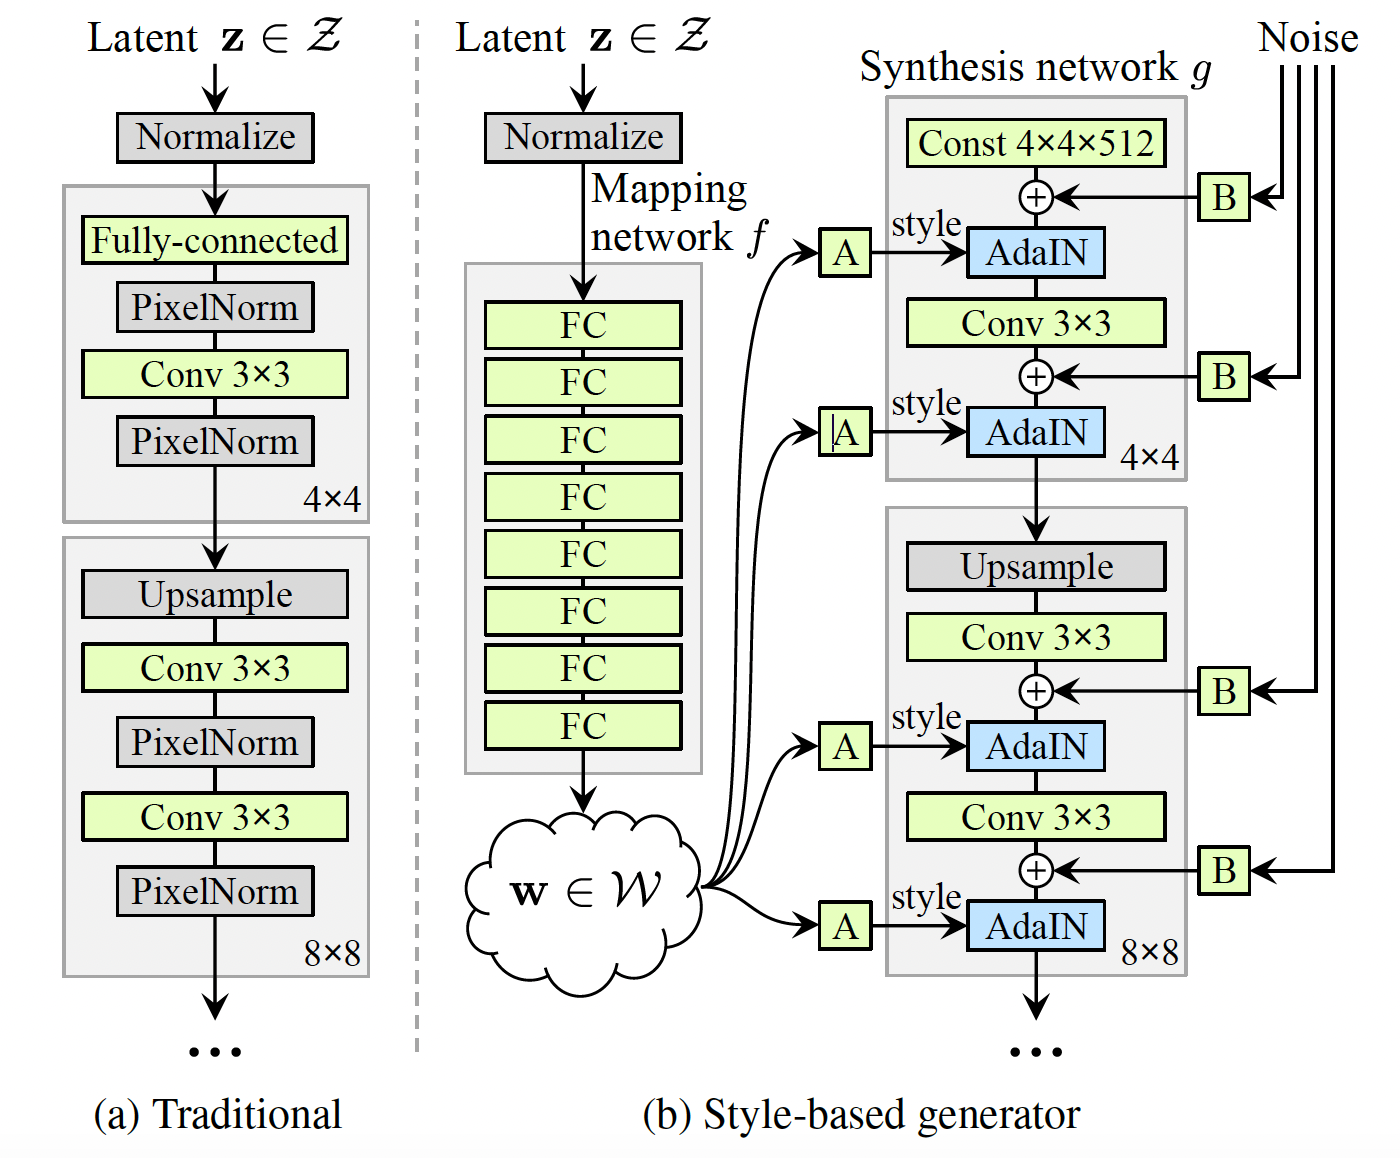
\includegraphics[width=0.7\textwidth]{imagesfrompapers/StyleGAN1arch.png} % Adjust the width as needed (e.g., 0.7\textwidth)
    \caption{StyleGAN Architecture. Figure from paper \cite{karras2019stylebased}}
    \label{styleganarch}
\end{figure}

\subsection{About the disentanglement of $\mathcal{W}$}

Unlike $\mathcal{Z}$ which has a fixed distribution ($\mathcal{N}(0, I_d)$), $\mathcal{W}$ has a distribution learned from $\mathcal{Z}$ and the authors claim that there is pressure from the generator for $\mathcal{W}$ to become more linear and therefore more disentangled.

\begin{comment}
    That pressure would come from the fact that it would be easier for the synthesis network to generate realistic images with a disentangled latent space than with an entangled latent space. That efficiency would come from the fact that it is easier for the linear unit $A$ that take a $w$ and apply a linear transformation before going into each AdaIN. This linear transformation has much more efficiency in a disentangled space.
\end{comment}

\subsection{About AdaIN operations}

As AdaIN is a transfer style operation (see Appendix \ref{Normalization}) it is remarkable that it is used at many different sizes of the image.

\subsection{About Noise}

This is a per-pixel Gaussian Noise, repeated for each channel.
It allows stochastic variations at different levels of details (as it operates at different steps of the generation) but above all it allows textures of thin details like hair. % "hair" is uncountable



\section{GANSpace}

\subsection{Presentation}

GANSpace \cite{harkonen2020ganspace} is a method that allows editing attributes of face images generated by StyleGAN by modifying their latent vectors $w \in \mathcal{W}$. The authors of \cite{harkonen2020ganspace} claim that the controls discovered by their method are interpretable. The method essentially relies on a principal component analysis (PCA) of the intermediate latent space $\mathcal{W}$. The exact procedure is as follows:

\begin{itemize}
    \item Randomly sample $N$ latent codes $(z_i)_{1 \leq i \leq N} \in \mathcal{Z}^N$ and compute their mappings $(w_i = f(z_i))_{1 \leq i \leq N} \in \mathcal{W}^N$.
    \item Perform a principal component analysis on the $w_i$, yielding $K \leq \min(d = 512, N)$ principal components $(\mathbf{v}_k)_{1 \leq k \leq K} \in (\mathbb{R}^d)^K$ and explained variances $\sigma_1^2 \geq ... \geq \sigma_K^2$. These will be our edit directions.
    \item Editing an image with intermediate latent code $w \in \mathcal{W}$:
    \begin{itemize}
        \item Select a principal component $k \in \{1, ..., K\}$ and an edit distance $\alpha \in \mathbb{R}$.
        \item Run the synthesis network using as input intermediate latent vector $w + \alpha \sigma_k \mathbf{v}_k$.

        Alternatively, select a set of layers $L \subset \{1, 2, ..., 18\}$ to which we want to apply our edit, and run the synthesis network using as input $w + \alpha \sigma_k \mathbf{v}_k$ for the layers in $L$ and $w$ for the other layers.
    \end{itemize}
\end{itemize}

Applying edits only to certain layers allows to perform editing of attributes at a desired scale only: editing the topmost layers will affect high-level attributes such as pose and face shape, while editing further layers will affect lower-level attributes such as hair color.

\subsection{Experiments and reproducibility}

We implemented GANSpace on the official PyTorch implementation of StyleGAN2 available at \url{https://github.com/NVlabs/stylegan2-ada-pytorch}. The PCA was performed using $N = \numprint{100000}$ samples (lower values of $N$ such as $N = \numprint{10000}$ turned out to provide unreliable principal components, \emph{i.e.} the principal components would change between iterations).

We tried editing faces using the principal components and layer groups mentioned in various places in the GANSpace paper \cite{harkonen2020ganspace}, and tried to find other interesting edition directions. We will reuse the following notations from the GANSpace paper: $V = \begin{pmatrix} \mathbf{v}_1 & ... & \mathbf{v}_{512} \end{pmatrix}^\top$ denotes the matrix of principal components of $\mathcal{W}$, $\mathrm{E}(\mathbf{v}_i, j-k)$ denotes the edition of layers $j$ to $k$ (inclusive) along principal component $\mathbf{v}_i$, $\mathrm{E}(\mathbf{v}_i, \mathrm{all}$ denotes edition of all layers along principal component $\mathbf{v}_i$ and $\mathrm{E}(\mathbf{v}_i, L)$ where $L \subset \{0, 1, ..., 17\}$ is a set of layers denotes edition of the layers in $L$ along principal component $\mathbf{v}_i$.

\begin{figure}[hbt!]
    \centering
    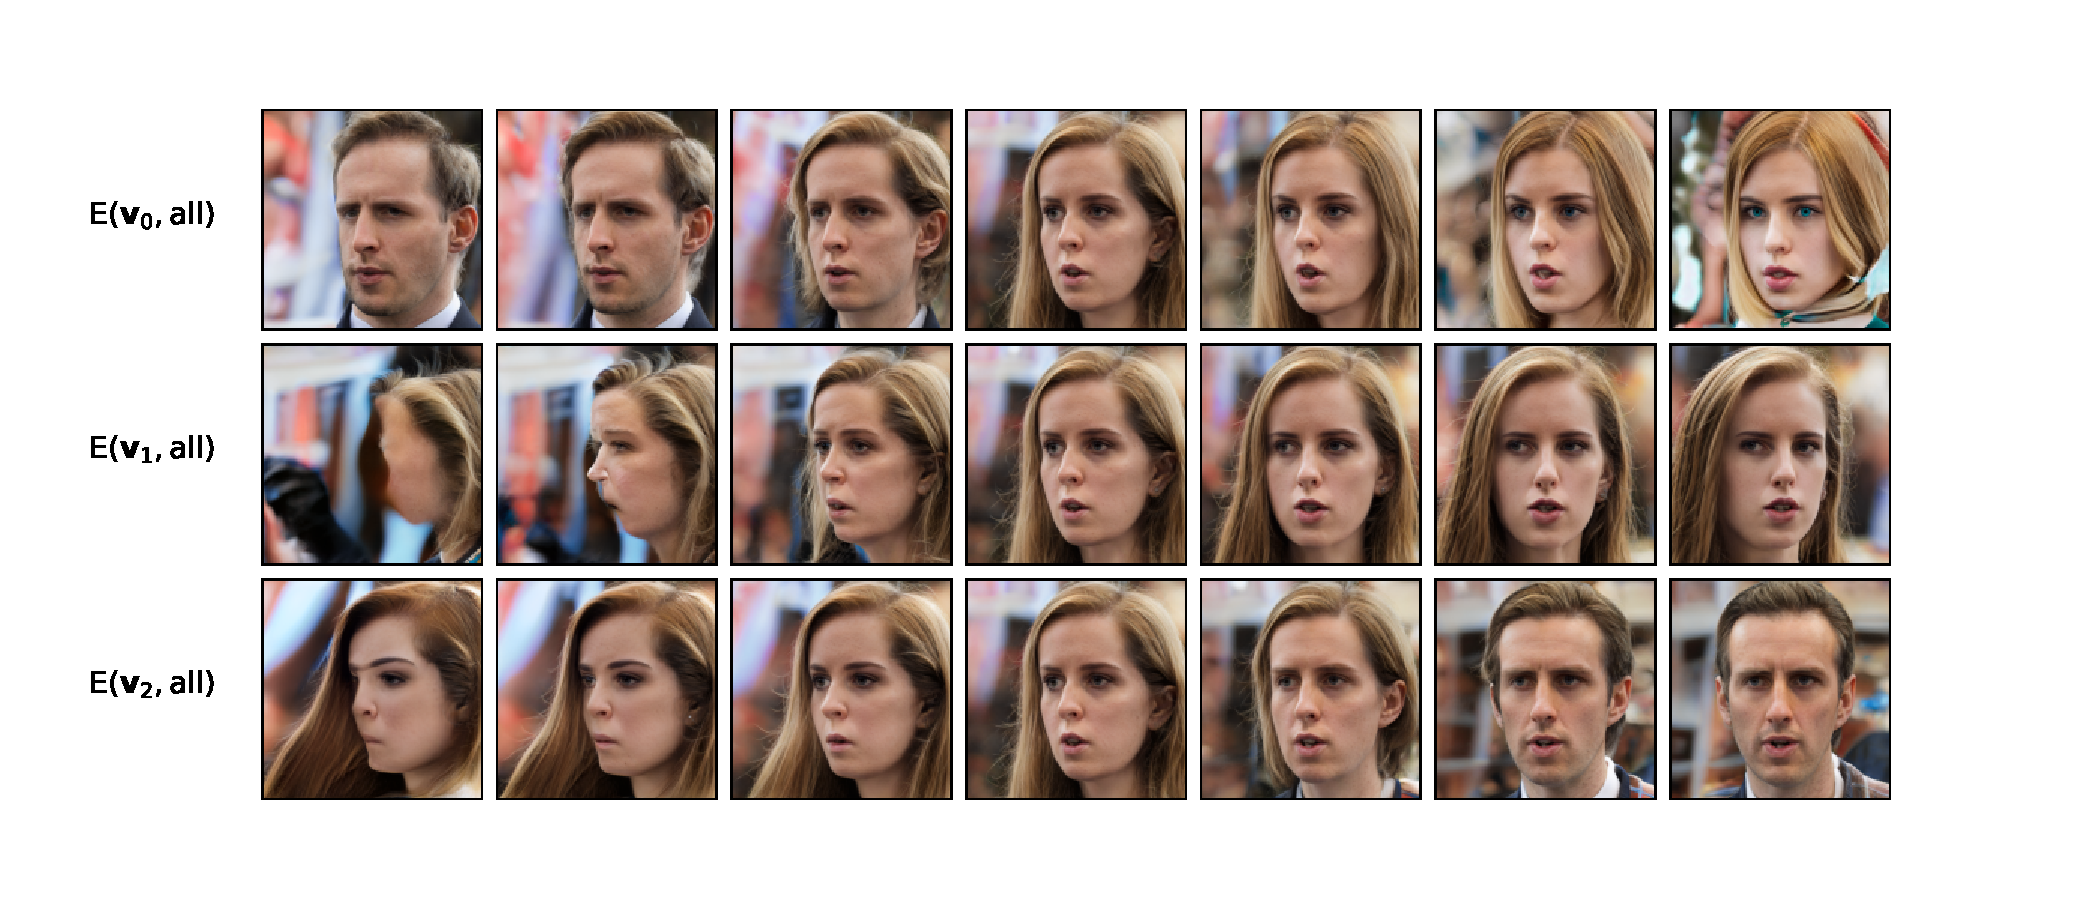
\includegraphics[width=\textwidth,trim={1.5cm 1cm 3cm 1cm},clip]{fig/all_components_1.pdf} \\
    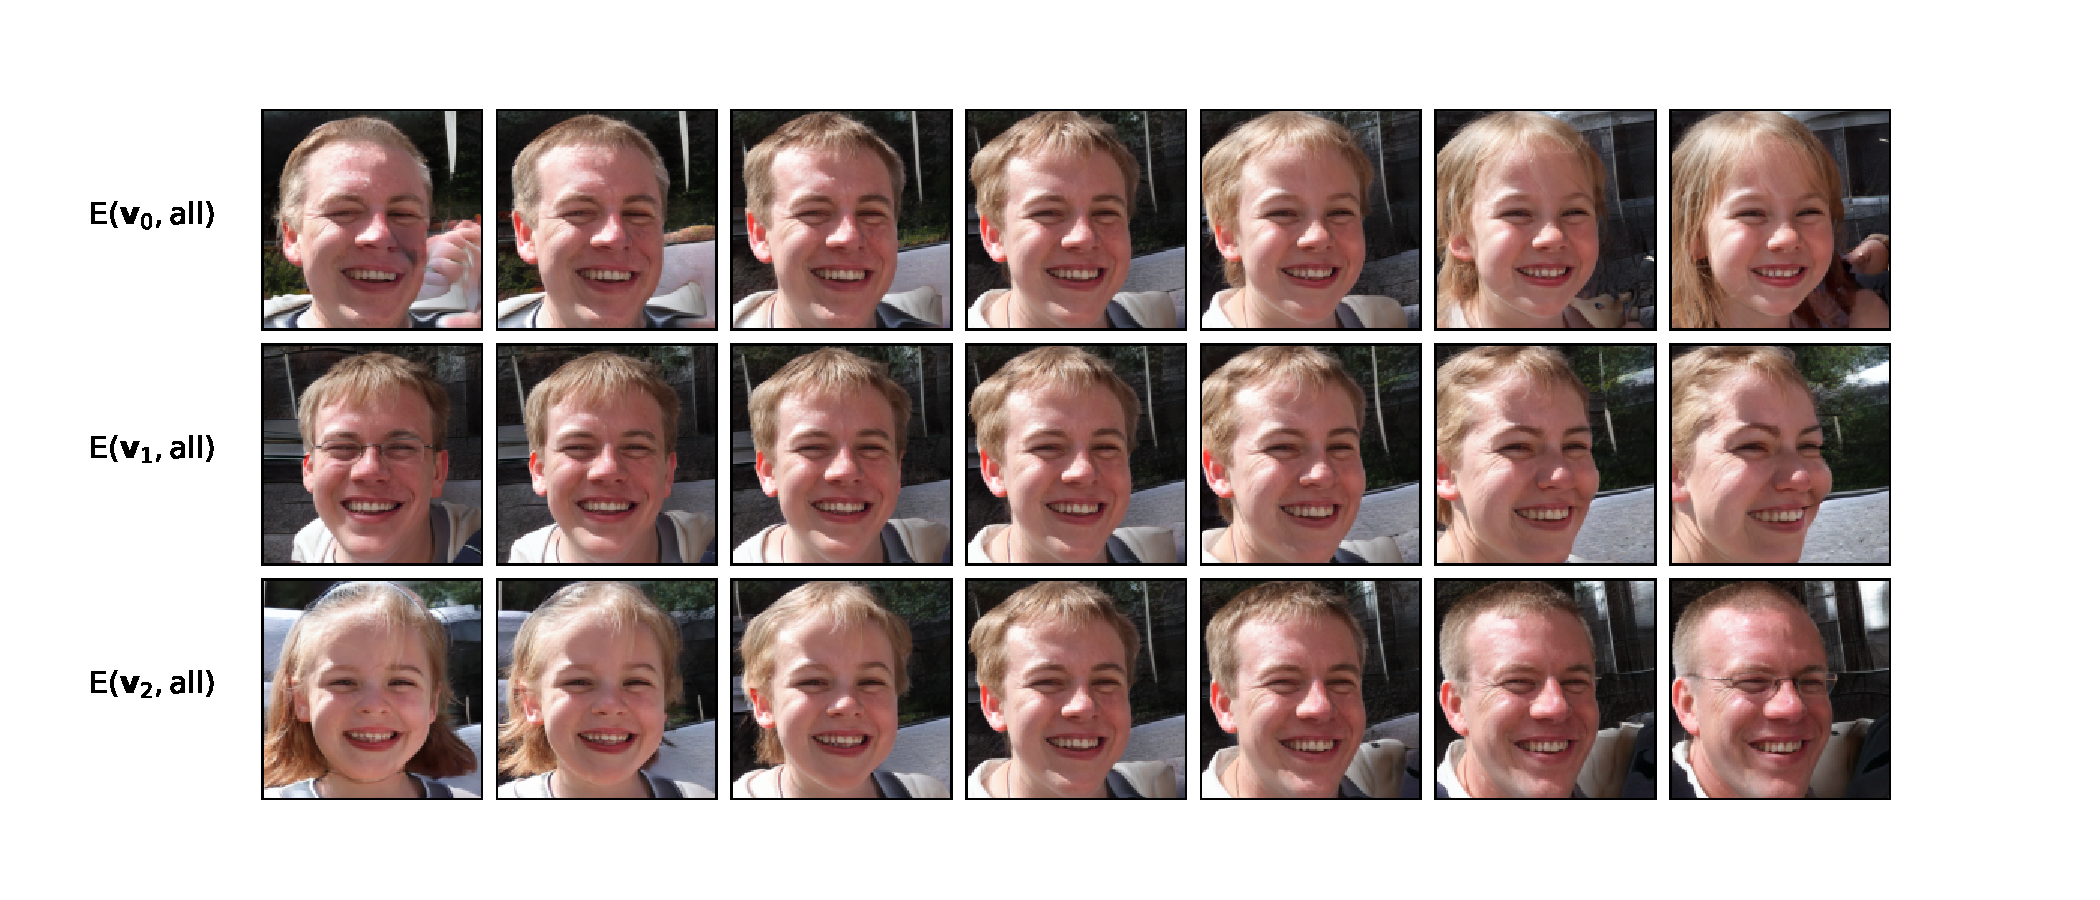
\includegraphics[width=\textwidth,trim={1.5cm 1cm 3cm 1cm},clip]{fig/all_components_2.pdf}
    \caption{Editing on all layers along components $\mathbf{v}_0$ to $\mathbf{v}_2$. Left: $-2\sigma$, right: $+2\sigma$.}
    \label{fig:all_components}
\end{figure}

Figure \ref{fig:all_components} shows the result of editing along the first three principal components on all layers. We observe behaviour that is rather consistent with what is stated in the GANSpace paper: editing along component $\mathbf{v}_0$ changes gender among other things, editing along component $\mathbf{v}_1$ changes face rotation and (less clearly) gender, and editing along component 2 changes rotation (sometimes not very clearly), age (often not very clearly), gender and background.

\begin{figure}[hbt!]
    \centering
    \begin{tikzpicture}
        \node[anchor=south west,inner sep=0] at (0, 0) {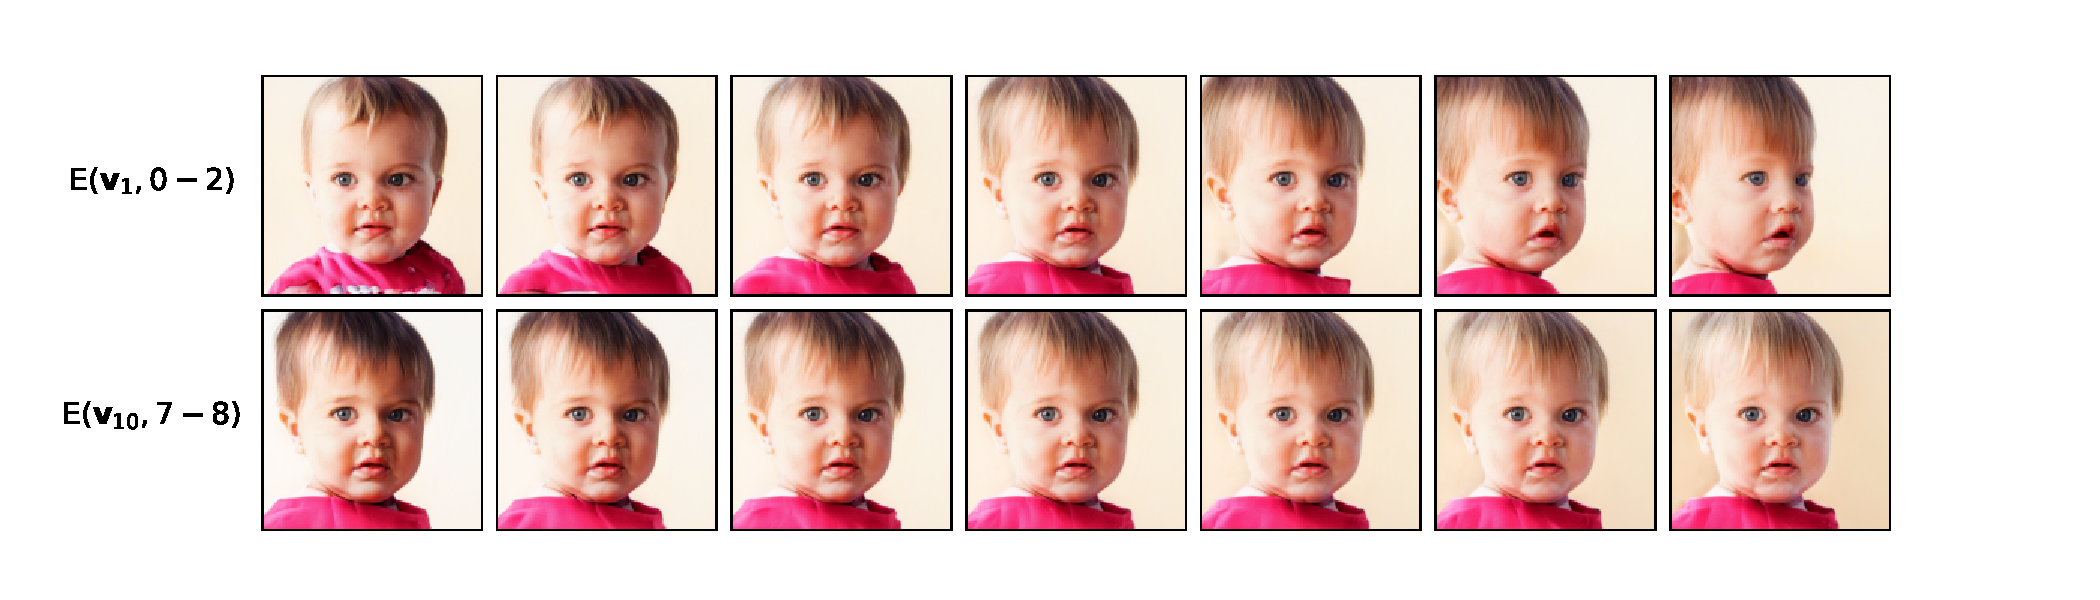
\includegraphics[width=.95\textwidth,trim={1cm 1cm 3cm 1cm},clip]{fig/layerwise_2.pdf}};
        \node[anchor=center] (mostlyrotate) at (0.5, 2.6) {\small mostly rotate};
        \node[anchor=center] (haircolor) at (0.75, 0.7) {\small hair color};
    \end{tikzpicture} \\
    \begin{tikzpicture}
        \node[anchor=south west,inner sep=0] at (0,0) {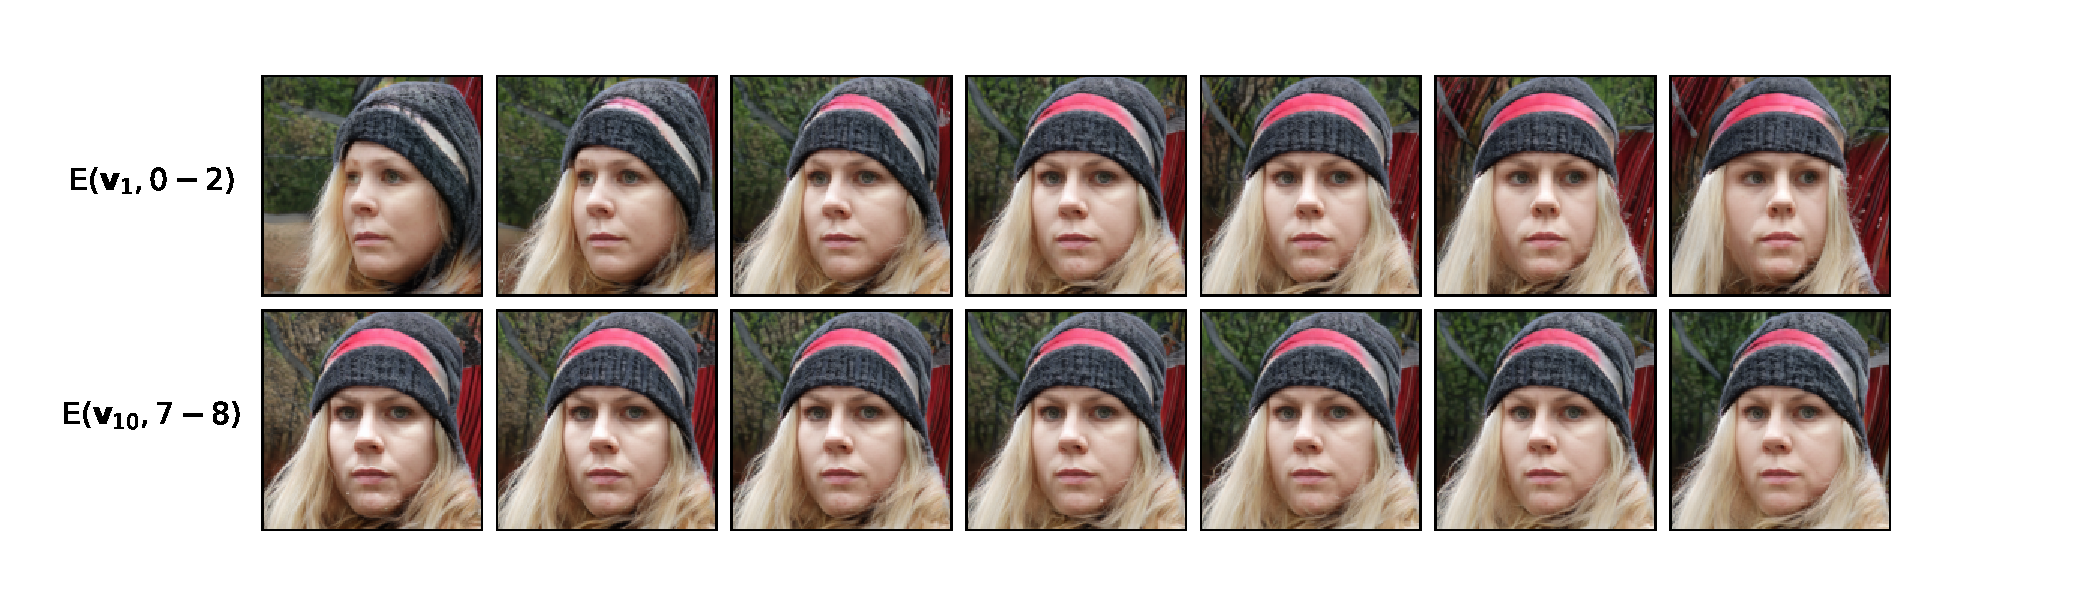
\includegraphics[width=.95\textwidth,trim={1cm 1cm 3cm 1cm},clip]{fig/layerwise_1.pdf}};
        \node[anchor=center] (mostlyrotate) at (0.5, 2.6) {\small mostly rotate};
        \node[anchor=center] (haircolor) at (0.75, 0.7) {\small hair color};
    \end{tikzpicture} \\
    \begin{tikzpicture}
        \node[anchor=south west,inner sep=0] at (0, 0) {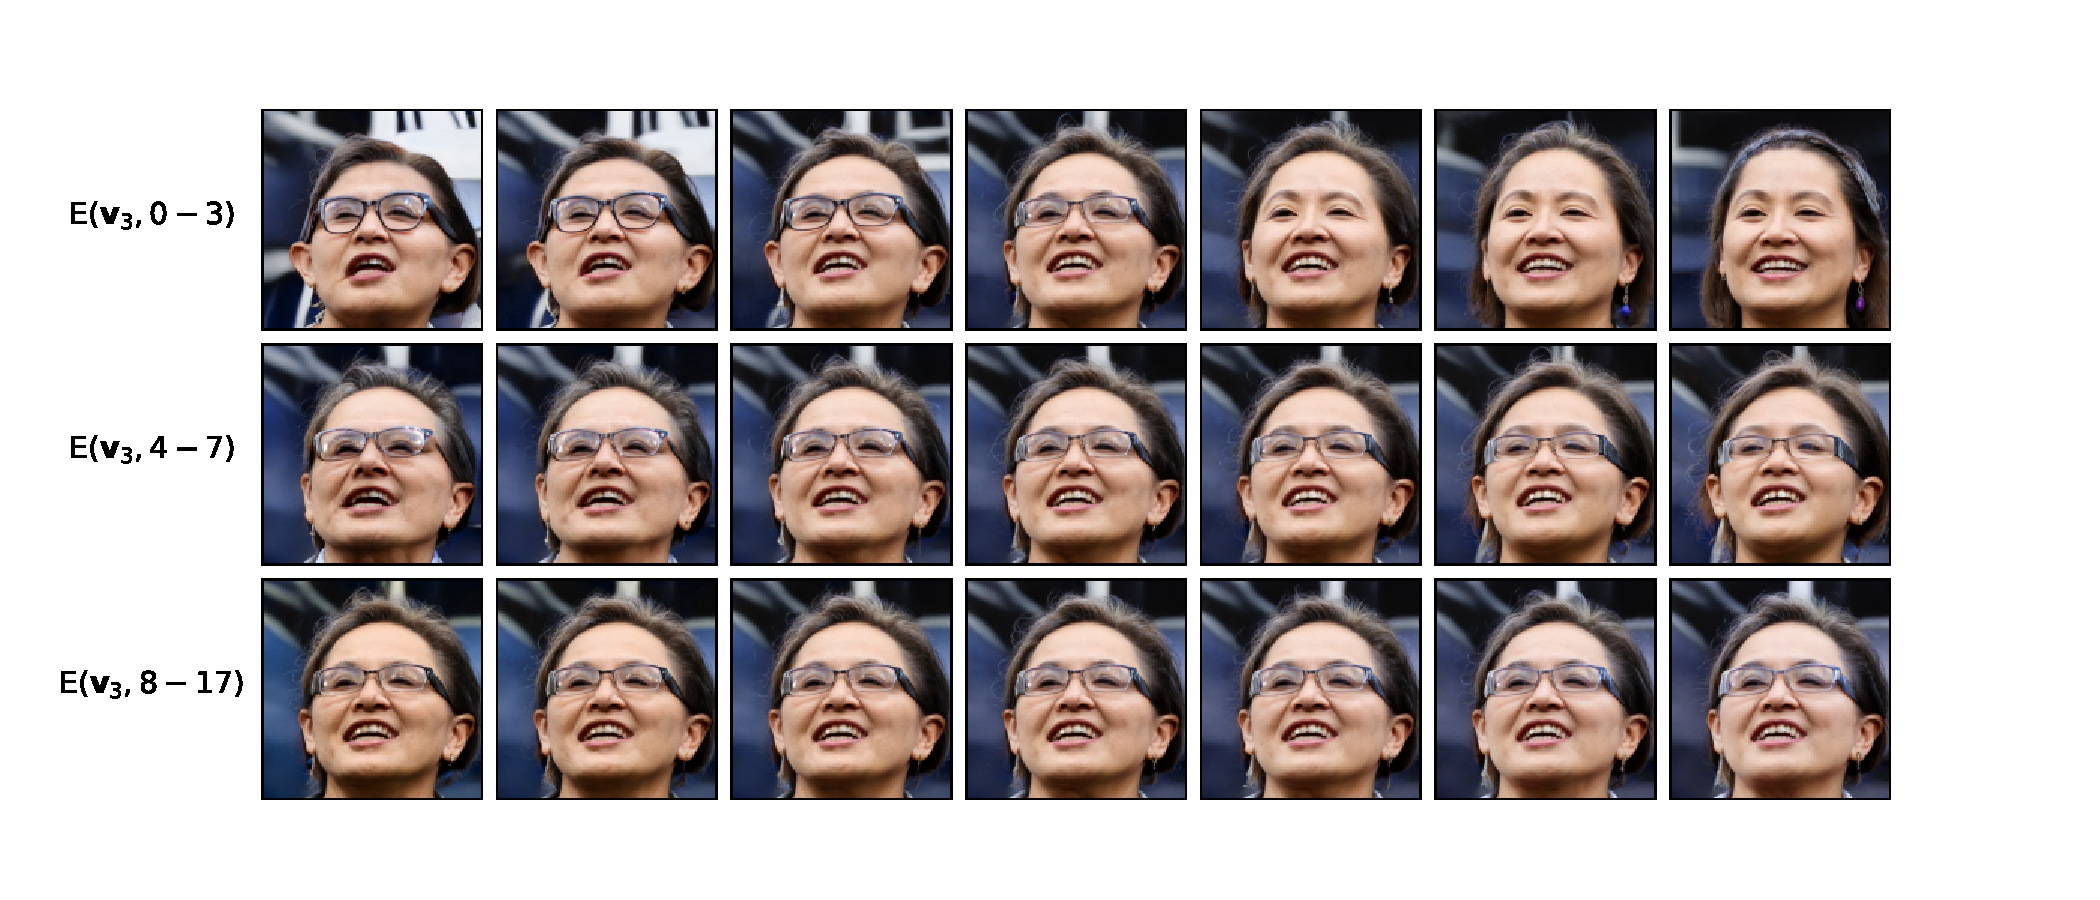
\includegraphics[width=.95\textwidth,trim={1cm 5.5cm 3.5cm 1.5cm},clip]{fig/layerwise_3.pdf}};
        \node[anchor=north,align=center] (glasses_maybe_age) at (0.7, 2.9) {\footnotesize glasses (and\\\footnotesize maybe age?)};
        \node[anchor=north,align=center] (age_gender) at (0.5, 0.9) {\footnotesize age and gender};
    \end{tikzpicture} \\
    \begin{tikzpicture}
        \node[anchor=south west,inner sep=0] at (0, 0) {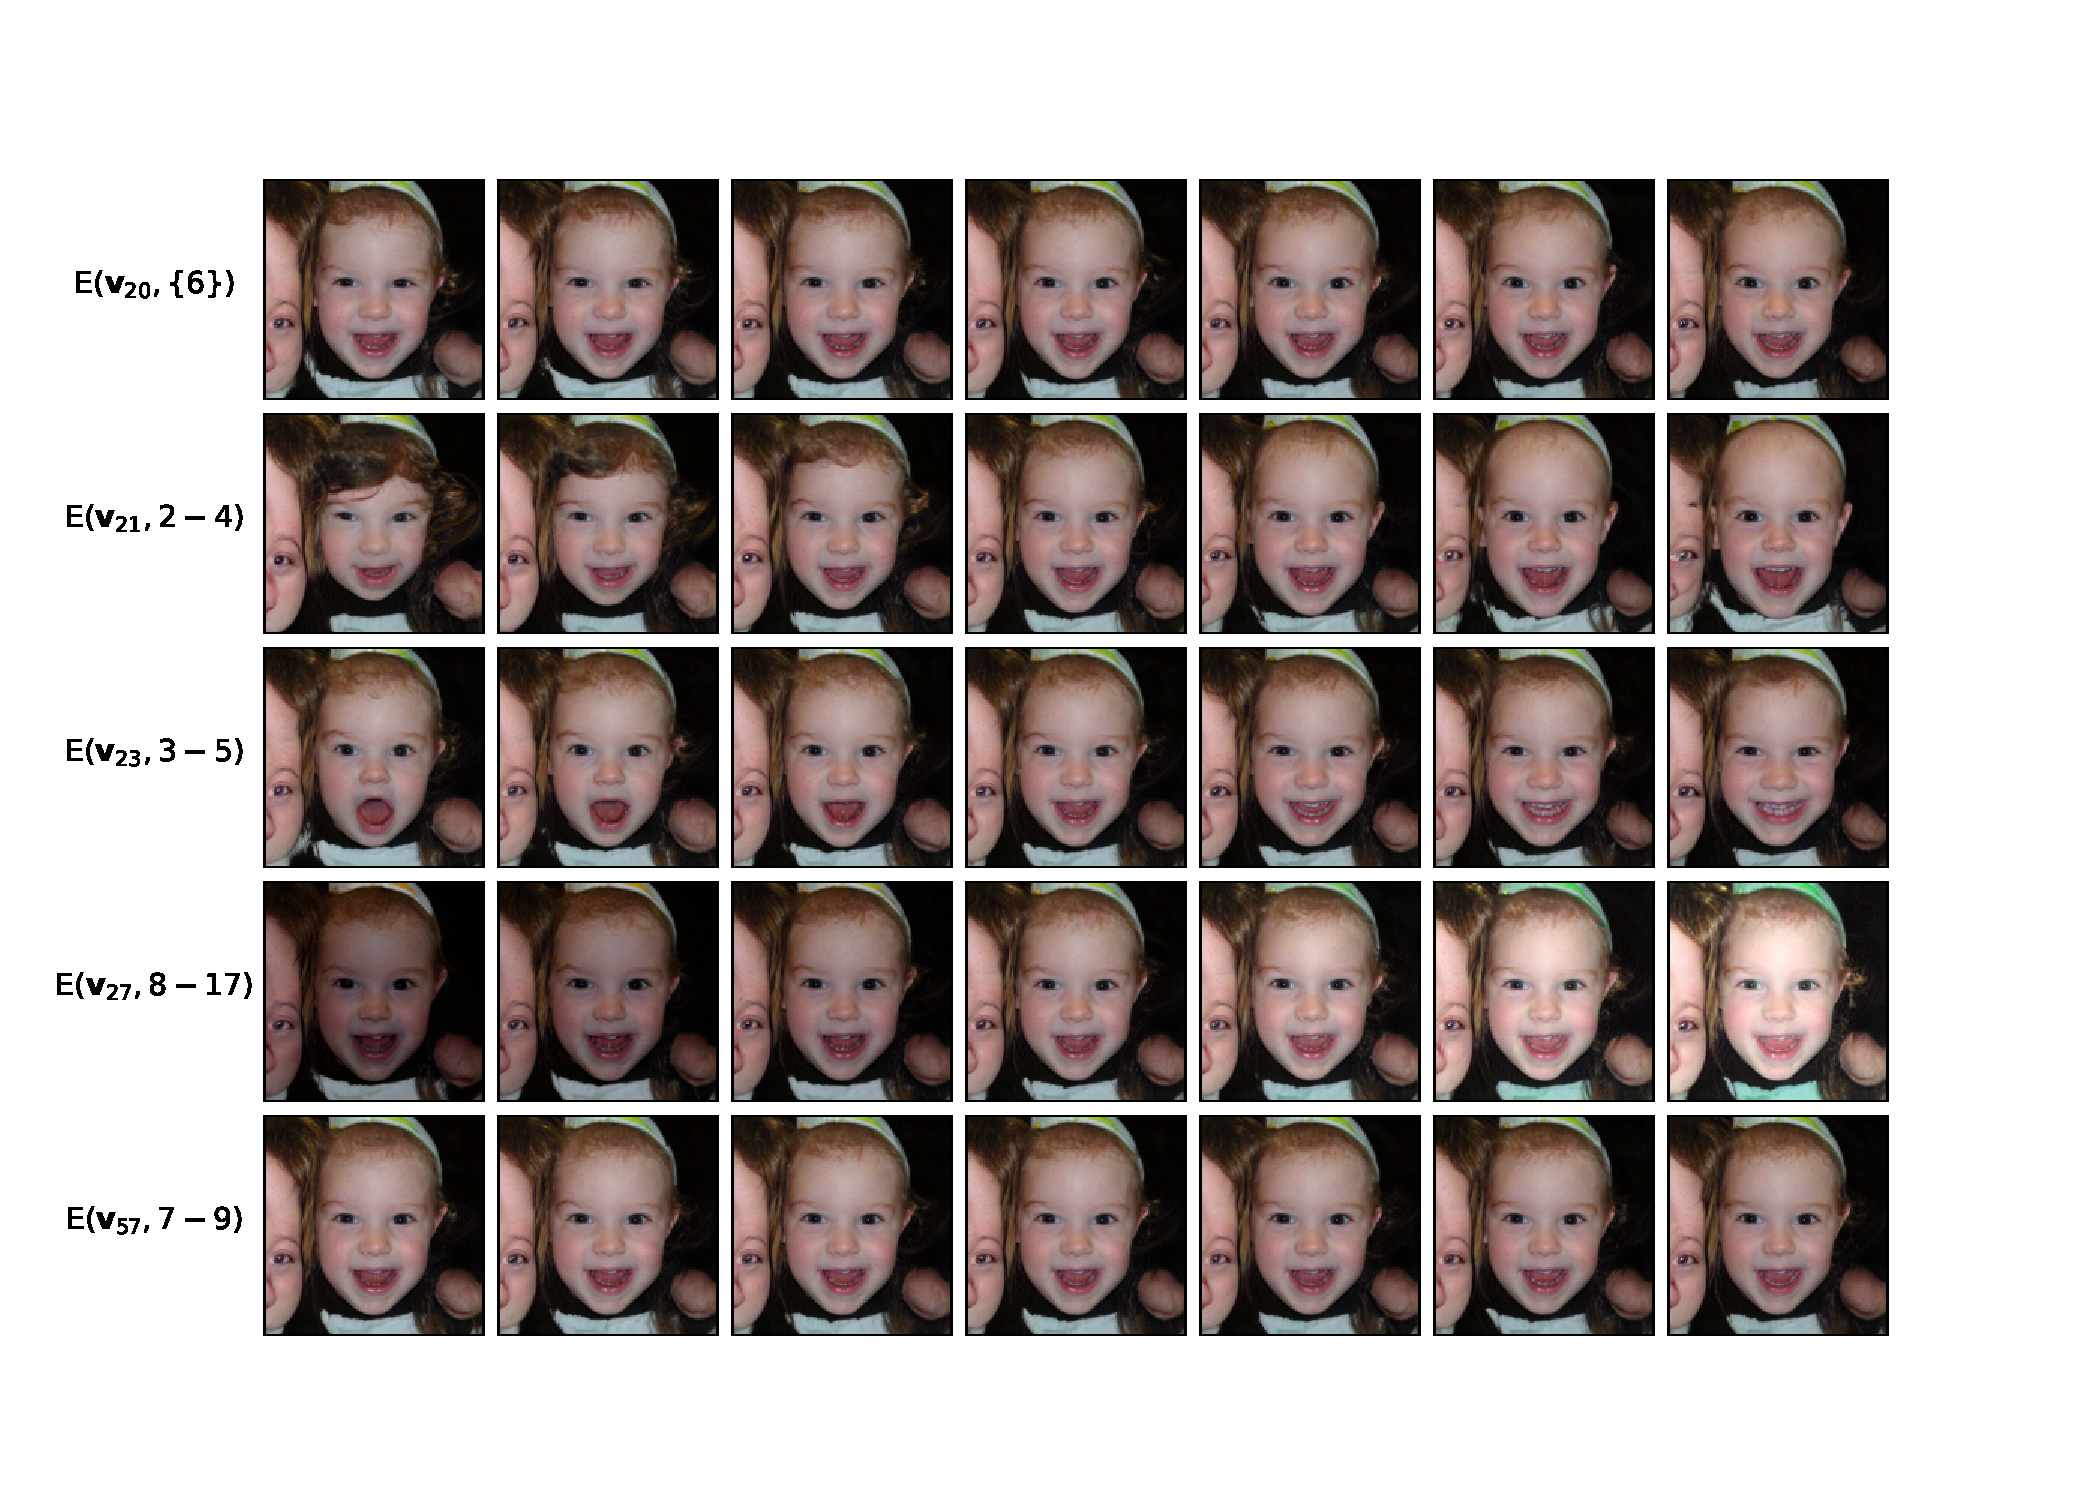
\includegraphics[width=.95\textwidth,trim={1cm 2.75cm 3.5cm 2.75cm},clip]{fig/layerwise_4.pdf}};
        \node[anchor=north,align=center] (wrinkles) at (0.8, 8.6) {\footnotesize wrinkles};
        \node[anchor=north,align=center] (baldness) at (0.8, 6.7) {\footnotesize baldness};
        \node[anchor=north,align=center] (expression) at (0.7, 4.8) {\footnotesize expression};
        \node[anchor=north,align=center] (exposure) at (0.75, 2.8) {\footnotesize exposure};
        \node[anchor=north,align=center] (white_hair) at (0.75, 0.9) {\footnotesize white hair};
    \end{tikzpicture}
    \caption{Editing of face images with various combinations of layers and principal components. The two examples using component $\mathbf{v}_3$ come from us, all other combinations come from the GANSpace paper \cite{harkonen2020ganspace}. \\
    Left: $-2\sigma$, right: $+2\sigma$.}
    \label{fig:layerwise}
\end{figure}

Figure \ref{fig:layerwise} shows the result of editing along a number of combinations of layers and principal components, most of which come from the GANSpace paper, but also with some that we found by ourselves.

We found that some attributes were more reliably edited than others. For instance, while edit $\mathrm{E}(\mathbf{v}_{27}, 8-17)$ corresponding to exposure looks very reliable and edit $\mathrm{E}(\mathbf{v}_1, 0-2)$ corresponding to rotation seems quite reliable, edit $\mathrm{E}(\mathbf{v}_{10}, 7-8)$ corresponding to hair color does not always succeed (see 4\textsuperscript{th} row of Fig. \ref{fig:layerwise}), and neither does edit $\mathrm{E}(\mathbf{v}_{20}, \{6\})$ (corresponding to wrinkles), at least for faces that are not expected to have wrinkles. It is however remarkable that the edit directions seem to apply to many unrelated images, and overall, we found the results of the GANSpace paper to be mostly reproducible.

Table \ref{tab:attributes_components} summarizes the most reliable GANSpace edit directions that either the authors of the GANSpace paper or we found.

\begin{table}[hbt!]
    \centering
    \begin{tabular}{l|l|l}
        \thead{Edit direction} & \thead{Attribute(s)} & \thead{Corresponding CelebA attribute \\ and attribute number} \\
        \hline
        $\mathrm{E}(\mathbf{v}_0, \mathrm{all})$ & Gender (among others) & \texttt{Male} (20) \\
        $\mathrm{E}(\mathbf{v}_1, \mathrm{all})$ & Rotate \& gender & \texttt{Male} (20) \\
        $\mathrm{E}(\mathbf{v}_2, \mathrm{all})$ & Rotate, age, gender, background & \texttt{Young} (39), \texttt{Male} (20) \\
        $\mathrm{E}(\mathbf{v}_{35}, \mathrm{all})$* & Mouth open & \texttt{Mouth\_Slightly\_Open} (21) \\
        $\mathrm{E}(\mathbf{v}_{36}\text{ or }\mathbf{v}_{37}, \mathrm{all})$* & Eyes closed & \\
        $\mathrm{E}(\mathbf{v}_{0}, 4-5)$* & Gender? & \texttt{Male} (20) \\
        $\mathrm{E}(\mathbf{v}_0, 6-17)$* & Age? & \texttt{Young} (39) \\
        $\mathrm{E}(\mathbf{v}_1, 0-2)$ & Mostly rotate & \\
        $\mathrm{E}(\mathbf{v}_2, 4-7)$* & Gender \& age & \texttt{Male} (20), \texttt{Young} (39) \\
        $\mathrm{E}(\mathbf{v}_3, 0-3)$* & Age \& glasses & \texttt{Young} (39), \texttt{Eyeglasses} (15) \\
        $\mathrm{E}(\mathbf{v}_{10}, 7-8)$ & Hair color (blond-brown?) & \texttt{Blond\_hair} (9), \texttt{Brown\_hair} (11) \\
        $\mathrm{E}(\mathbf{v}_{16}, 8-17)$* & Hair color (black/brown/blond?) & \texttt{Black\_hair} (8), \texttt{Brown\_hair} (11), \texttt{Blond\_hair} (9) \\
        $\mathrm{E}(\mathbf{v}_{17}, 4-7)$* & Mouth slightly open? & \texttt{Mouth\_Slightly\_Open} (21) \\
        $\mathrm{E}(\mathbf{v}_{20}, \{6\})$ & Wrinkles & \\
        $\mathrm{E}(\mathbf{v}_{21}, 2-4)$ & Bald & \texttt{Bald} (4) \\
        $\mathrm{E}(\mathbf{v}_{23}, 3-5)$ & Facial expression (smiling) & \texttt{Smiling} (31) \\
        $\mathrm{E}(\mathbf{v}_{27}, 8-17)$ & Overexpose & \\
        $\mathrm{E}(\mathbf{v}_{57}, 7-9)$ & White hair & \texttt{Gray\_hair} (17)
    \end{tabular}
    \caption{Non-exhaustive list of GANSpace edit directions and associated CelebA attributes (if any). * denotes edit directions found by us, the other directions come from the GANSpace paper.}
    \label{tab:attributes_components}
\end{table}

\section{Comparison with other methods}

\subsection{Presentation of InterFaceGAN}
\label{subsect:interfacegan_pres}

InterFaceGAN \cite{shen2020interfacegan} is another method for editing face images in the latent space of StyleGAN. It makes use of an (approximate) linear separability hypothesis and an external face image classifier.

The main steps of the algorithm are as follows:
\begin{itemize}
    \item Generate a dataset of $N$ randomly sampled images from the considered GAN.
    \item Extract a subset of the dataset for each feature that we wish to edit, and label this subset with two labels: positive or negative. For instance, using a classifier for a feature, label the top \numprint{10000} scored samples with positive and the last \numprint{10000} with negative.
    \item Train a SVM on each of these labeled subsets to obtain a separating hyperplane for each of them.
    \item Edit a sample $z$ from the latent space as follows:
    If $n$ is a unit vector defining the hyperplane of a feature, compute $z_{edit} = z + \alpha n$ where $\alpha \in \mathbb{R}$.
\end{itemize}
Contrary to GANSpace which can only be applied to the intermediate latent space $\mathcal{W}$, this method can be applied to both the original latent space $\mathcal{Z}$ with Gaussian distribution and the intermediate latent space $\mathcal{W}$. We implemented InterFaceGAN on the PyTorch implementation of StyleGAN2 (available at \url{https://github.com/NVlabs/stylegan2-ada-pytorch}, same as for GANSpace), restricting ourselves to the intermediate latent space $\mathcal{W}$.

\begin{comment}
Liste des attributs dans l'ordre: 
\begin{minted}[breaklines]{text}
['5_o_Clock_Shadow', 'Arched_Eyebrows', 'Attractive',
'Bags_Under_Eyes', 'Bald', 'Bangs', 'Big_Lips', 'Big_Nose',
'Black_Hair', 'Blond_Hair', 'Blurry', 'Brown_Hair', 'Bushy_Eyebrows',
'Chubby', 'Double_Chin', 'Eyeglasses', 'Goatee', 'Gray_Hair',
'Heavy_Makeup', 'High_Cheekbones', 'Male', 'Mouth_Slightly_Open',
'Mustache', 'Narrow_Eyes', 'No_Beard', 'Oval_Face', 'Pale_Skin',
'Pointy_Nose', 'Receding_Hairline', 'Rosy_Cheeks', 'Sideburns',
'Smiling', 'Straight_Hair', 'Wavy_Hair', 'Wearing_Earrings',
'Wearing_Hat', 'Wearing_Lipstick', 'Wearing_Necklace',
'Wearing_Necktie', 'Young']
\end{minted}
\end{comment}

\subsection{Comparison with GANSpace}

To compare GANSpace with InterFaceGAN, we proceeded as follows. We generate a test dataset of $N_{test} = \numprint{10000}$ images. We then select a number of attributes that can be edited both by using GANSpace and by using InterFaceGAN: we settled on baldness (attribute \#4), gender (\#20) and smiling (\#31). For each chosen attribute, we create two subsets of images corresponding to the top $p\%$ scores ("positive images") and the lowest $p\%$ scores ("negative images"; we chose $p = 2$). We then edit the resulting subsets in order to try to make the positive images look negative and vice-versa. Finally, we run the attribute classifier on the resulting edited images and compute the average score as well as a success rate based on a score threshold that we determine manually (by looking at randomly sampled images with their scores).

\subsubsection*{Determining the edit distance $\alpha$}

As mentioned in section \ref{subsect:interfacegan_pres}, we need to choose an edit distance $\alpha \in \mathbb{R}$ when considering $z_{edit} = z + \alpha n$. The vector $n$ has the property that for each labeled sample $(z_i, y_i)$,

$$ y_i(n^\top z_i + b) \geq 1-\zeta_i $$ for some $\zeta_i \geq 0$ that is hopefully small enough and some $b \in \mathbb{R}$ (intercept of the hyperplane, independent of $i$).

When editing an image with latent code $z$ towards the positive label, one way of choosing the edit distance is first (orthogonally) projecting $z$ onto the separating hyperplane, then adding a fixed edit distance $\alpha_0$ that does not depend on the input image (but may depend on the chosen attribute). This amounts to choose:

$$ \alpha = \frac{-n^\top z - b}{||n||^2} + \alpha_0 $$

\begin{figure}[hbt!]
    \centering
    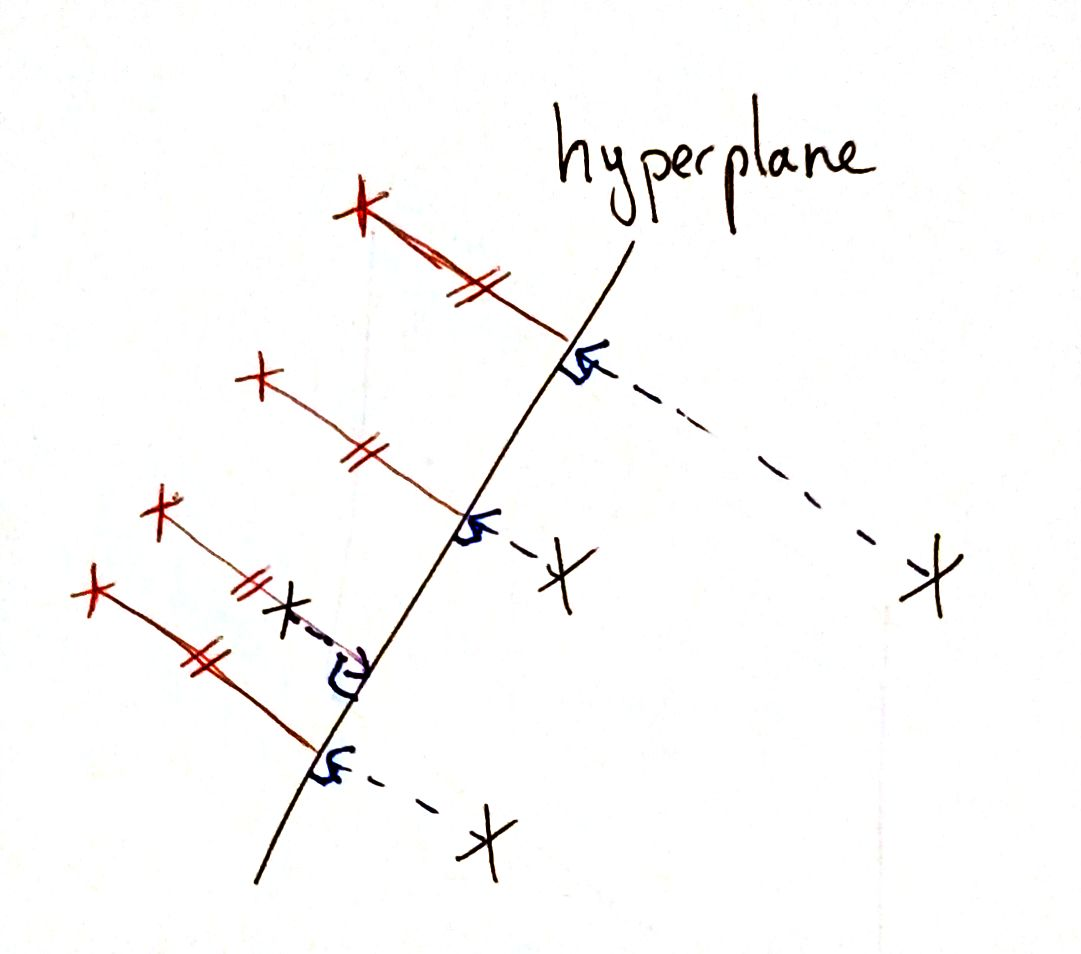
\includegraphics[width=.4\textwidth]{fig/Hyperplane.jpg}
    \caption{Illustration of our method for choosing the edit distance $\alpha$ in InterFaceGAN.}
    \label{fig:hyperplane}
\end{figure}

See Fig. \ref{fig:hyperplane} for an illustration of this method. We used this method for our benchmarks, since it allows to control the distance of the output image to the hyperplane, making it independent of the position of the input latent code to the hyperplane. The authors of the InterFaceGAN paper \cite{shen2020interfacegan} use a constant as $\alpha$ instead.

\subsubsection{Experiments}

We ran few experiments, you can see the gender edition in Fig. \ref{ifganexp}.

We can see that the editions are much less entangled than the ones with GANSpace, a lot attribute : smile, glasses, expression, hair color etc. are the same during the passage from a gender to another. \\ We also may notice that the discriminator is not so perfect, especially for the last two scores in the first and last rows, where we can see two similar faces to human eyes even though their scores are very different. This is also a reminder that gender involves a significant element of subjectivity and is therefore perhaps not the best feature to study rigorously.

\begin{figure}[hbt!]
    \centering
    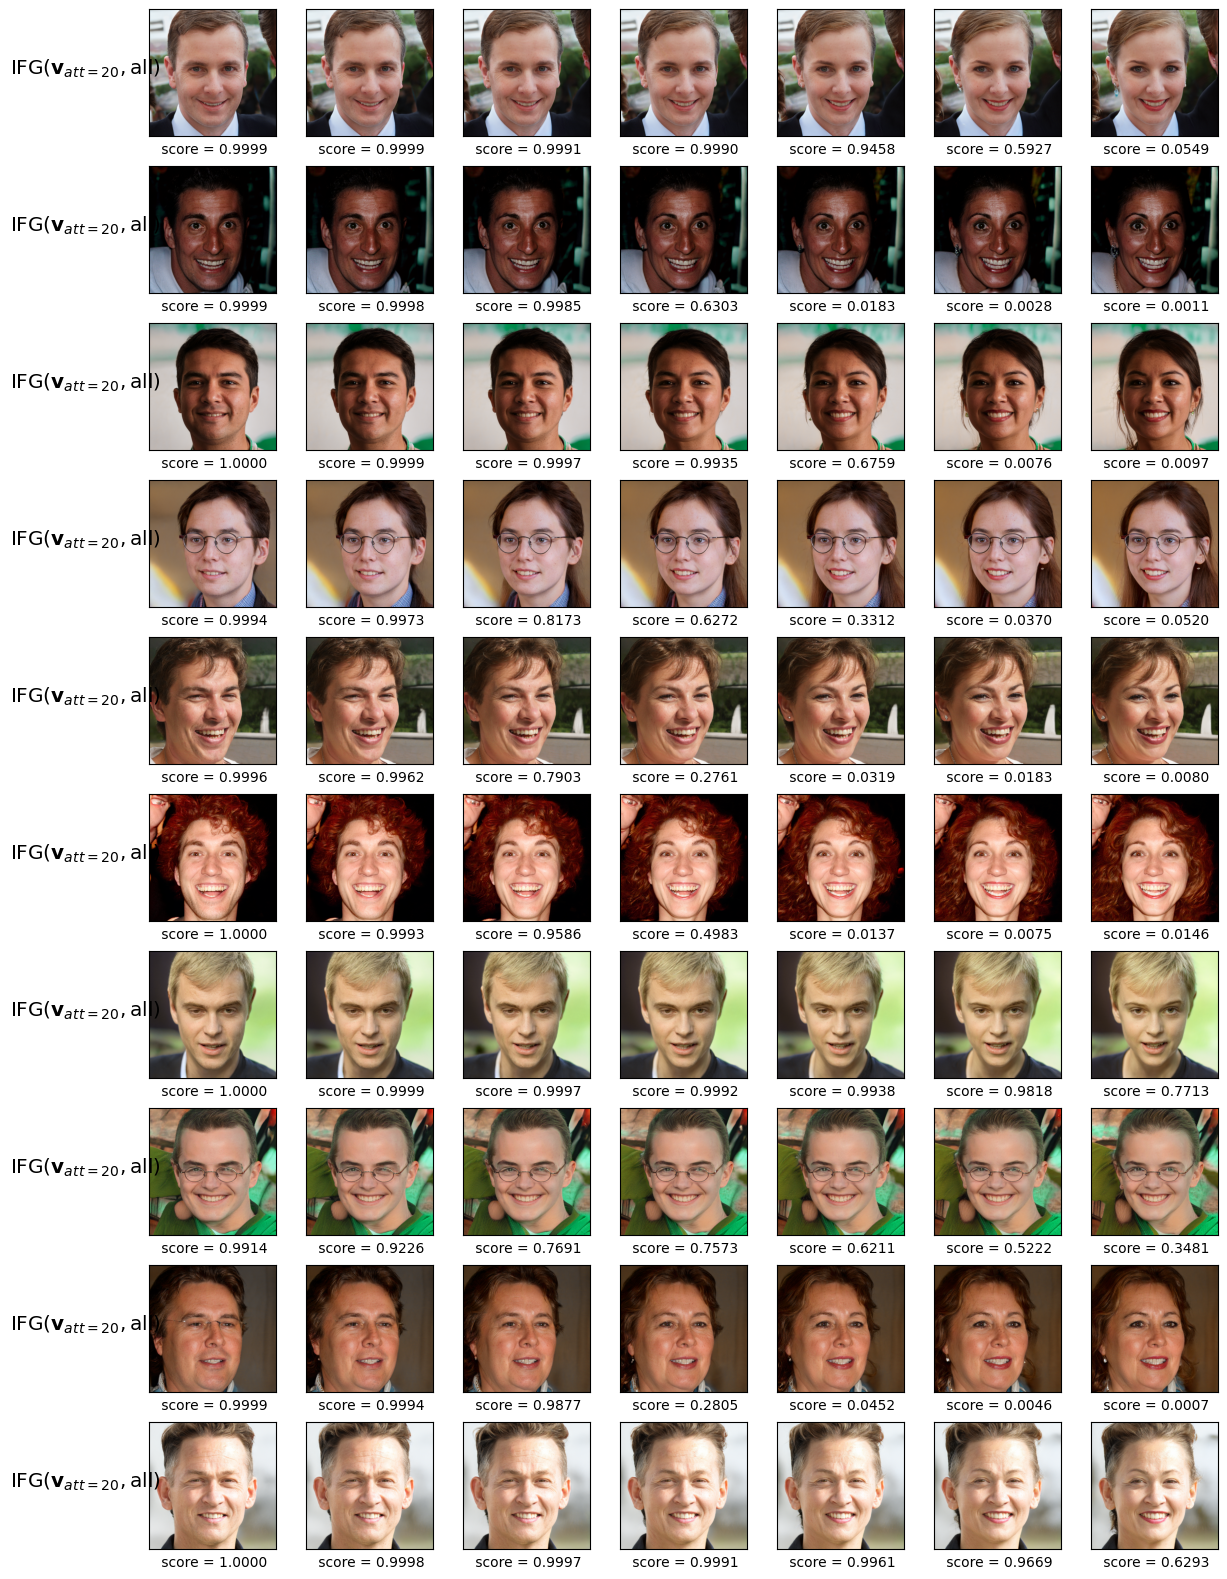
\includegraphics[width=\hsize]{fig/IFGANgenderwscore.png}
    \caption{Gender edition with InterFaceGAN, from male towards female (1 towards -1). The score is the one of same discrimnator used to label our datasets.}
    \label{ifganexp}
\end{figure}

We also ran for smiling edition in Fig. \ref{ifganexp2}. Here the discriminations are much clearer and without debate, we can notice again the quality of disentanglement of that edition.

\begin{figure}[hbt!]
    \centering
    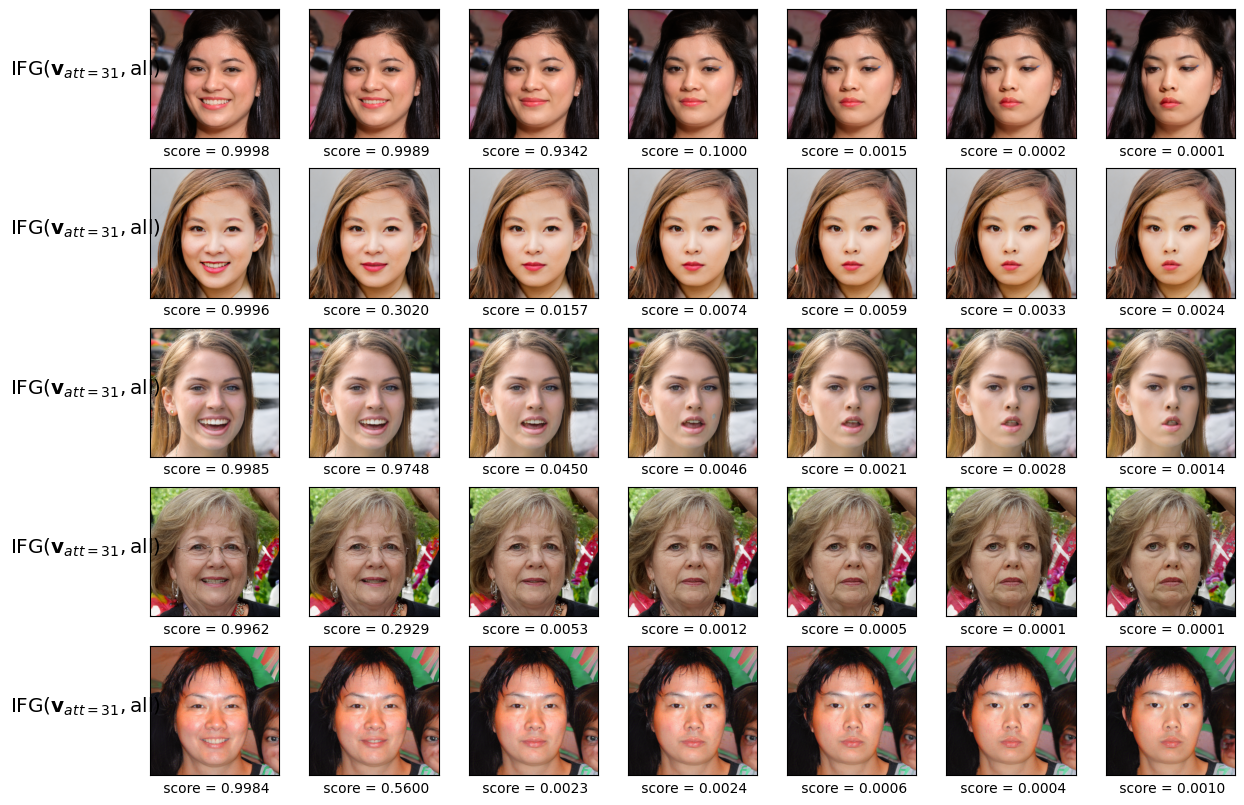
\includegraphics[width=\hsize]{fig/IFGANSmileTounsmile.png}
    \caption{Smile edition with InterFaceGAN, from smiling towards non-smiling (1 towards -1). The score is the one of same discrimnator used to label our datasets.}
    \label{ifganexp2}
\end{figure}
\subsubsection*{Results}

\begin{table}[hbt!]
    \centering
    \begin{tabular}{lrrrr}
    \hline
     IFGAN, attribute 31 (smiling)      &   average &    std &   accuracy &   threshold \\
    \hline
     direction : 1 towards -1 &   0.00054 & 0.0011 &      1     &       0.015 \\
     direction : -1 towards 1 &   0.98345 & 0.0783 &      0.985 &       0.73  \\
    \hline
    \hline
     GANSpace, attribute 31 (smiling)   &   average &    std &   accuracy &   threshold \\
    \hline
     direction : 1 towards -1 &   0.28832 & 0.4041 &      0.37  &       0.015 \\
     direction : -1 towards 1 &   0.67801 & 0.3923 &      0.635 &       0.73  \\
    \hline
    \hline
     IFGAN, attribute 4 (bald)       &   average &    std &   accuracy &   threshold \\
    \hline
     direction : 1 towards -1 &   0.0092  & 0.0695 &      0.965 &       0.018 \\
     direction : -1 towards 1 &   0.19556 & 0.3327 &      0.145 &       0.62  \\
    \hline
    \hline
     GANSpace, attribute 4 (bald)    &   average &    std &   accuracy &   threshold \\
    \hline
     direction : 1 towards -1 &   0.01896 & 0.0753 &      0.79  &       0.018 \\
     direction : -1 towards 1 &   0.26215 & 0.3291 &      0.185 &       0.62  \\
    \hline
    \hline
     IFGAN, attribute 20 (male)      &   average &    std &   accuracy &   threshold \\
    \hline
     direction : 1 towards -1 &   0.26261 & 0.3444 &      0.605 &        0.12 \\
     direction : -1 towards 1 &   0.71332 & 0.391  &      0.565 &        0.95 \\
    \hline
    \hline
     GANSpace, attribute 20 (male)   &   average &    std &   accuracy &   threshold \\
    \hline
     direction : 1 towards -1 &   0.15803 & 0.2508 &       0.7  &        0.12 \\
     direction : -1 towards 1 &   0.91329 & 0.2574 &       0.87 &        0.95 \\
    \hline
    \end{tabular}
    \caption{Performance of InterFaceGAN (IFGAN) and GANSpace for three face attributes.}
    \label{tab:performance}
\end{table}

Results are presented in Table \ref{tab:performance}. % TODO Comment

We note that the performance of GANSpace for baldness (attribute 4) seems to be particularly bad for the direction -1 to 1, with an average score of only around 0.26. We made an observation on the classifier that may partly explain this bad performance. Figure \ref{fig:discri_bias} shows the result of editing some images to make the faces more bald using GANSpace ($\mathrm{E}(\mathbf{v}_{21}, 2-4)$), along with the scores (after sigmoid) of each image by the classifier for the attribute \texttt{Bald} (4). All five examples visually look like successful edits, but we note that the classifier fails to classify the images of bald \emph{women} as bald. We hypothesize that the training dataset of the classifier is biased towards male bald faces, because bald female faces are less common in reality than male bald faces.

Other than that, we note that InterFaceGAN seems to work significantly better than GANSpace, with respective accuracies of over 98\% and between 37\% and 64\%. However, InterFaceGAN seems to perform slightly worse for editing gender, with lower success rates than for GANSpace. We hypothesize that this is because edits with InterFaceGAN are more disentangled than those of GANSpace, resulting in edits that only apply the minimum changes needed to change the gender of any given face, something that the classifier may not have picked up effectively.

\begin{figure}[hbt!]
    \centering
    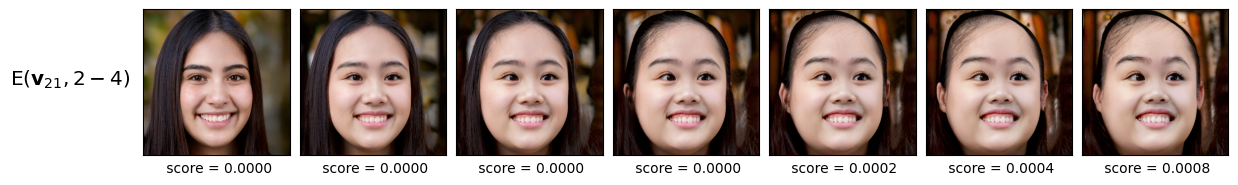
\includegraphics[width=\hsize]{fig/DiscriBias1.png}
    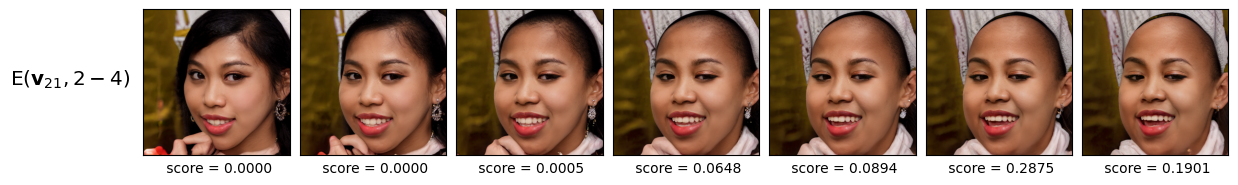
\includegraphics[width=\hsize]{fig/DiscriBias2.png}
    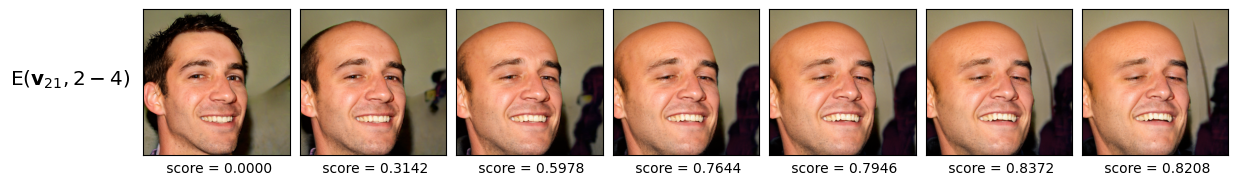
\includegraphics[width=\hsize]{fig/DiscriBias3.png}
    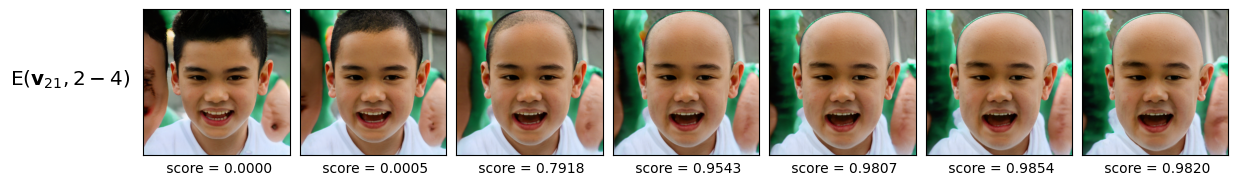
\includegraphics[width=\hsize]{fig/DiscriBias4.png}
    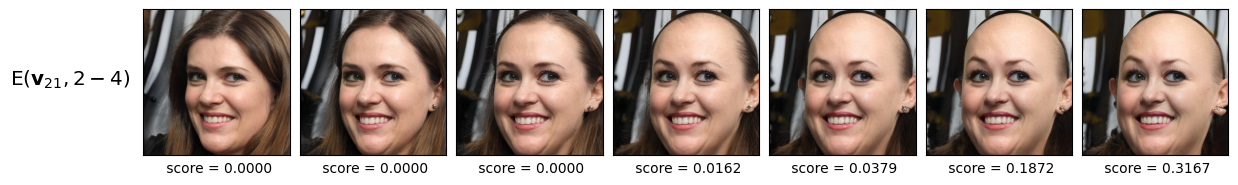
\includegraphics[width=\hsize]{fig/DiscriBias5.png}
    \caption{Examples of face edits towards bald faces using GANSpace (original image on the left, right: $+50\sigma$). The numbers below each image are the scores (after sigmoid) of the image by the attribute classifier for attribute \texttt{Bald} (4).}
    \label{fig:discri_bias}
\end{figure}

\section{Possible future work}

We thought of a number of possibilities of future work on the project, which we did not explore due to lack of time and computing resources (since we only used Google Colab's free GPUs).

\begin{itemize}
    \item One could consider using a face identification model to evaluate whether GANSpace and InterFaceGAN edits change the identity of the edited images. This metric would partially reflect the disentanglement of the intermediate latent space of StyleGAN.
    \item We did not have time to study the disentanglement of the intermediate latent space $\mathcal{W}$ compared to the original latent space $\mathcal{Z}$. One idea that we had was to use the classifier to quantify how attributes are entangled with each other, by editing an image along one direction (given by GANSpace or InterFaceGAN) and quantifying the variation of the other scores by the classifier, either by computing the correlation of the score of the edited attribute with the other scores, or by computing the sum of absolute differences in one given score (to account for the possibility that, for instance, when editing a face to be more bald, the face changes gender twice, which would be a sign of entanglement of the considered latent space). This second idea is actually a variant of the perceptual path length metric defined in the StyleGAN paper \cite{karras2019stylebased}, where we replace the metric based on VGG16 embeddings with a metric based on the attribute classifier.
    \item We were limited in the quality and quantity of our calculations due to the lack of computational resources (free Google Colab only). For instance, during the process of applying InterFaceGAN to StyleGAN2, when creating the two labeled subsets of images for each attribute in order to run a SVM on the resulting labeled dataset, we restricted ourselves to $N = \numprint{15000}$ samples and considered the samples with the top $10\%$ and lowest $10\%$ instead of $2\%$ (as the authors of the InterFaceGAN paper \cite{shen2020interfacegan} did). As a consequence, for attributes where the positive (resp. negative) images are under-represented, negative (resp. positive) images may end up being labeled as positive (resp. negative), adversely affecting the quality of the SVM. When comparing GANSpace with InterFaceGAN, we limited ourselves to $N_{test} = \numprint{10000}$ total samples, however we did use the images with the top and lowest 2\% scores.
    \item We could have compared GANSpace and InterFaceGAN on more attributes (we identified 7 attributes that could be edited by both methods, see Table \ref{tab:attributes_components}), but we only did on 3 attributes.
    \item We did not try applying InterFaceGAN on the original latent space $\mathcal{Z}$.
    \item We did not use the truncation trick, i.e. pass the argument \texttt{truncation\_psi = 0.7} to \texttt{G.mapping}. This trick brings latent codes closer to the barycenter of $\mathcal{W}$, leading to more stable generation and less artefacts. This could have improved the quality of the SVM of InterFaceGAN.
    \item The idea would be to make a large number of edits with different scale factors ($\alpha$) and combinations of layers and components, then send the images to the classifier and finally examine the distribution of each edit direction in the classifier results.
\end{itemize}

\begin{comment}

Mesurer si l'éditeur change la personne ou non grâce à un nouveau classifieur qu'on devrait trouver sur le net.

Chercher des directions d'édition à la main est assez laborieux, car l'édition échoue assez souvent.

L'implémentation "officielle" de GANSpace (\url{https://github.com/harskish/ganspace}) contient un outil interactif : l'utiliser pour trouver plus facilement des directions d'édition interprétables, en vue de comparer avec InterFaceGAN ?
\end{comment}

\section{Conclusion}

\begin{itemize}
    \item StyleGAN proves to be effective at providing a disentangled latent space as shown in the StyleGAN paper (perceptual path length metric) and by the effectiveness of both PCA and SVM for face image editing.
    \item GANSpace advantages : 
    \begin{itemize}
        \item The PCA is performed directly on latent vectors and hence does not require a resource-intensive generation and classification of images like the SVM of InterFaceGAN does.
        \item Simplicity of the algorithm, only needs a PCA and gives quite good results.
    \end{itemize}
    \item GANSpace drawbacks :
    \begin{itemize}
        \item There are a lot of components/layers  combinations making it quite long to identify what are the attributes we can edit.
        \item GANSpace "proposes" edit directions while IFGAN allows to select the attribute we want (as long as there is a classifyer for them).
        \item For instance, InterFaceGAN thanks to a good classifyer, instantly gives attribute edition and in a much less entangled way than the PCA. Indeed, the SVM gives more guarantee that the direction will edit as we want, PCA hasn't got a strong theory indicating that the the founded directions will be along attributes, neither that the founded attributes will be attribute that makes sense for human eyes.
        \item We can not take into account the position of the vector we edit. Unlike InterFaceGAN for instance.
    \end{itemize}
\end{itemize}

\section{Normalizations}\label{Normalization}

See the corresponding paper : \cite{huang2017arbitrary}.
\\\\Here is a presentation of three different normalizations, the one used in the StyleGAN is AdaIN.
\\\\The general principle of a normalization is to center and reduce with a certain mean $\mu(x)$ and variance $\sigma(x)$ where $x$ is the variable we want to normalize. Here $x$ will represent an image with some channels (possibly more than 3 as they are convolutions in the GANs) and a certain width $W$ and height $H$.

\subsection{Batch Normalisation (BN)}
The Batch Normalisation means that the mean and variance is computed through every pixels of every image of each batch, this is therefore the same one that will be applied to every pixels of every images.
\\\\N = batch size
\\X = batch of images
\\W, H = Width, Height of each image
\\ $x_{i,hw}$ = pixel of position (h,w) of the $i^{th}$ image.

\begin{equation}
    \mu(X) = \frac{1}{NHW}\sum_{i\text{\textsuperscript{th} image of batch}}\sum_{\text{position }(h, w)} x_{i, hw}
\end{equation}

\begin{equation}
    \sigma(X)^2 = \frac{1}{NHW}\sum (x_{ihw} - \mu(X_i))^2 
\end{equation}

\subsection{Instance Normalisation (IN)}

Here, instead of doing it batch-wise, we do it sample-wise. There are a couple (mean, variance) for each different images : 

\begin{equation}
    \mu_i(x_i) = \frac{1}{HW}\sum_{(h, w)\text{ position}} x_{hw}
\end{equation}
\begin{equation}
    \sigma(x_i)^2 = \frac{1}{HW}\sum (x - \mu(x_i))^2 
\end{equation}

\subsection{Adaptive Instance Normalisation (AdaIN)}
Adaptive Instance Normalization acts in two parts. It first does an instance normalisation, and then takes the mean and variance from another image and applies it to the current as follows : 

\begin{equation}
AdaIN(x, y) = \sigma(y) \left(\frac{x - \mu(x)}{\sigma(x)}\right) + \mu(y)
\end{equation}

\vspace{0.5cm}
Where x and y are single images, $\mu$ and $\sigma$ computed as in the instance normalisation.

The couple (mean, variance) from the other image is called the \textbf{style}.

This operation is supposed to transfer a style to another. In Figure \ref{2figs} is an example with two real images.

\begin{figure}[H]
  \centering
  \begin{subfigure}{.45\textwidth}
    \centering
    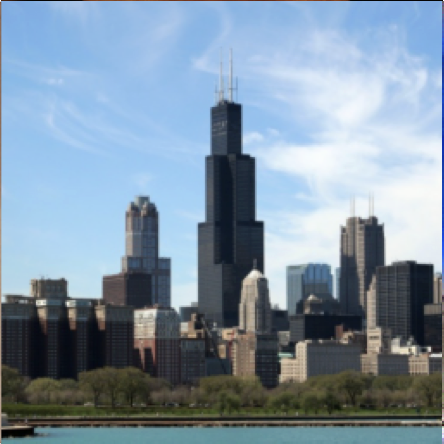
\includegraphics[width=\linewidth]{imagesfrompapers/content image.png}
    \caption{content image}
  \end{subfigure}%
  \begin{subfigure}{.45\textwidth}
    \centering
    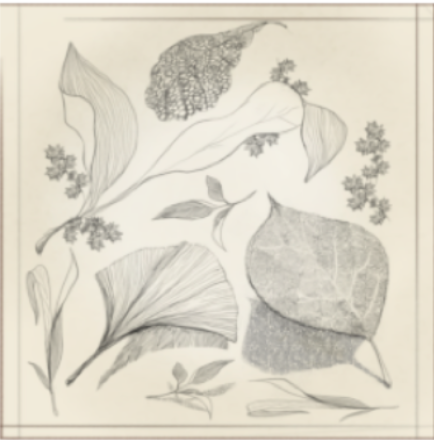
\includegraphics[width=\linewidth]{imagesfrompapers/style image.png}
    \caption{style image}
  \end{subfigure}
  \begin{subfigure}{.45\textwidth}
    \centering
    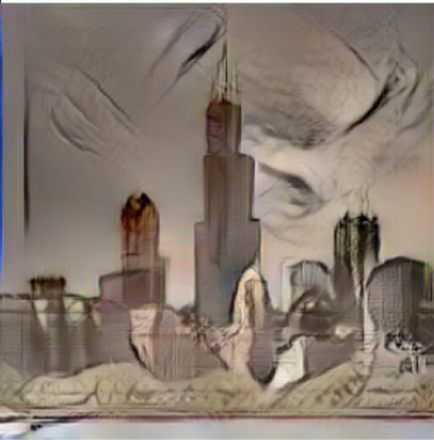
\includegraphics[width=\linewidth]{imagesfrompapers/AdaIN.png}
    \caption{AdaIN(content, style)}
  \end{subfigure}
  \caption{Example of style transfer by AdaIN. Pictures from this paper \cite{chandran2022adaptive} }
  \label{2figs}
\end{figure}


\bibliographystyle{plain}
\bibliography{bibliography}
\end{document}
